\documentclass[user_manual.tex]{subfiles}
\begin{document}

%Inicio de la introducción
\chapter{Introducción}

El manual de usuario tiene como propósito de servir como una guía clara y específica para garantizar el uso y funcionamiento óptimo de Justina ``el robot de servicio'', resolver las dudas más comunes sobre el robot; así como la posibilidad para desarrollar una replica del robot con fines de investigación. Comprende de la descripción general de los subsistemas de Justina.\\

Se contempla todo lo relacionado al hardware empleado y se provee de ligas para ver especificaciones más avanzadas; éstas son dadas para el lector interesado en una explicación más detallada.\\

Este documento contiene los algoritmos creados por los integrantes del laboratorio de biorobotica. Para cada modulo está incluida una breve descripción del algoritmo, técnicas o enfoques usados para el diseño.\\ %

El robot de servicio Justina fue diseñado en el laboratorio de Biorobotica de la facultad de ingeniería de la UNAM. Cabe señalar que este documento está sujeto a actualizaciones conforme sean requeridas por modificaciones hechas en el robot Justina.\\

En la figura \ref{fig:introduction:Justina} se muestra el robot de servicio Justina.

%Figura 1.1 de Justina
\begin{figure}[H]
\centering
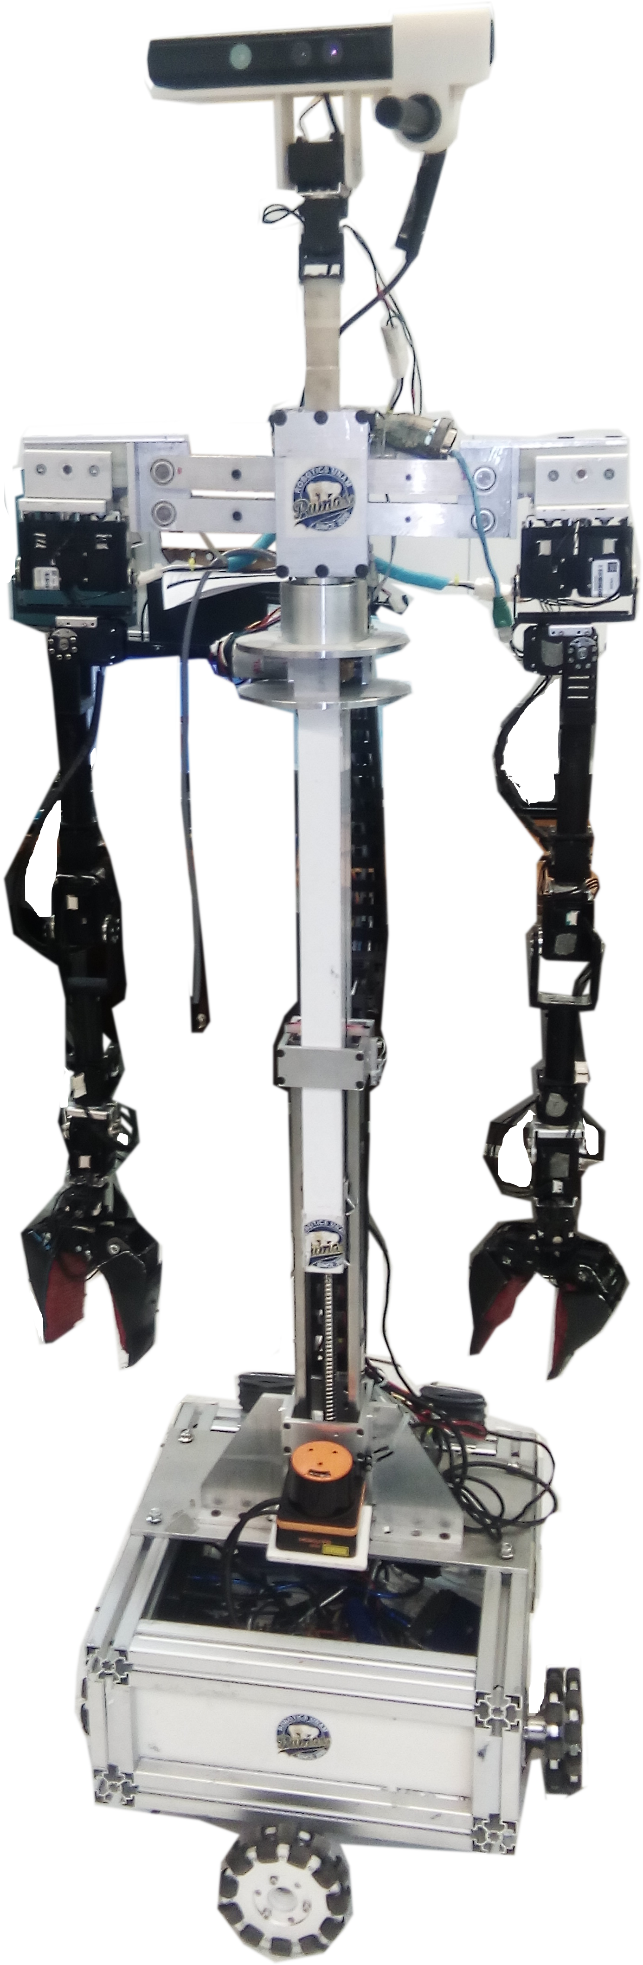
\includegraphics[width=0.7\textwidth]{Figures/Introduction/Justina.png}
\caption{El Robot Justina}
\label{fig:introduction:Justina}
\end{figure}
\pagebreak


\end{document}